\section{Usability Testing}
\subsection{การวางแผนการทดสอบ}
\begin{enumerate}
    % \item \textbf{Product under test}
    %       \begin{itemize}
    %         \item What's being tested?
    %         \item What are the business and experience goals of the product
    %       \end{itemize}
    \item \textbf{จุดประสงค์ของการทดสอบ}
          \begin{itemize}
              \item \textbf{เป้าหมายของการทดสอบ} : เพื่อวัดประสิทธิภาพการใช้งานของเว็ปแอพลิเคชันกับผู้ใช้
              \item \textbf{คำถามที่ใช้ในการทดสอบ} : เราได้เตรียมคำถามไว้ถามผู้ใช้หลังจากการทดสอบ โดยแบ่งคำถามออกเป็น 3 ประเภท ดังตาราง ดังนี้
                \begin{table}[H]
                    \caption{ตารางคำถามที่ใช้ในการทดสอบ}
                    \label{tab:question-table}
                    \begin{tabularx}{\textwidth}{|l|X|lll}
                    \cline{1-2}
                    \textbf{ประเภทคำถาม}                        & \textbf{คำถาม}                                                                                    &  &  &  \\ \cline{1-2}
                    \multirow[t]{5}{*}{ความเหมาะสมของวิธีแก้ปัญหา}       & Solution ที่เสนอแก้ปัญหาได้จริงไหม แก้ได้หมด หรือแก้ได้บางส่วน                                    &  &  &  \\ \cline{2-2}
                                                                & มีปัญหาหรือความต้องการอะไรอีกไหมที่ solution ยังไม่ตอบโจทย์                                       &  &  &  \\ \cline{2-2}
                                                                & ถ้าเทียบกับ solution อื่น ๆ ที่เคยใช้ คิดว่า solution นี้เป็นอย่างไร                              &  &  &  \\ \cline{2-2}
                                                                & มีองค์ประกอบไหนที่ควรเติมเพื่อทำให้ solution มีประสิทธิภาพมากขึ้นในการ แก้ปัญหา                   &  &  &  \\ \cline{2-2}
                                                                & มีข้อจำกัดอะไรในการนำไปใช้งานจริงสำหรับกลุ่มเป้าหมาย เช่น ต้นทุน เวลา ความง่ายในการใช้งาน เป็นต้น &  &  &  \\ \cline{1-2}
                    \multirow[t]{4}{*}{การใช้งาน} & Feature/function ไหนที่คิดว่าควรมี (แล้วยังไม่มี) หรือไม่จำเป็นต้องมี                             &  &  &  \\ \cline{2-2}
                                                                & Feature/function ไหนที่คุณคิดว่ามีประโยชน์หรือไม่มีประโยชน์                                       &  &  &  \\ \cline{2-2}
                                                                & ลองให้คะแนนภาพรวมของ functions ของ solution นี้  1-10                                             &  &  &  \\ \cline{2-2}
                                                                & ทำยังไงให้ fuctions ของ solution ได้คะแนนเต็ม 10                                                  &  &  &  \\ \cline{1-2}
                    \multirow[t]{5}{*}{ประสบการณ์ผู้ใช้}            & การใช้งาน solution ยาก/ง่ายอย่างไร เหมาะกับกลุ่มเป้าหมายไหม                                       &  &  &  \\ \cline{2-2}
                                                                & มีส่วนไหนของ solution ที่งงหรือใช้งานยาก                                                          &  &  &  \\ \cline{2-2}
                                                                & ชอบ solution/การใช้งานส่วนไหนมากที่สุด                                                            &  &  &  \\ \cline{2-2}
                                                                & ชอบ solution/การใช้งานส่วนไหนน้อยที่สุด                                                           &  &  &  \\ \cline{2-2}
                                                                & มีข้อเสนอแนะตรงไหนที่จะทำให้ประสบการณ์การใช้งาน solution ดีขึ้น                                   &  &  &  \\ \cline{1-2}
                    \end{tabularx}
                    \end{table}
              \item \textbf{สมมุติฐานที่ต้องการทดสอบ} : สมมุติฐานที่ต้องการทดสอบคือเรื่องการใช้งานของทั้ง 3 ฟีเจอร์ ดังนี้
              \begin{itemize}
                \item Career Prediction : สามารถช่วยทำให้ผู้ใช้เห็นแนวทางของเรซูเมตัวเองมากขึ้นว่าเป็นอาชีพไหน  
                \item Career Insight : สามารถเห็นภาพรวมอาชีพและแนะนำการพัฒนาเรซูเมว่าควรมีทักษะอะไรเพิ่ม 
                \item Career Exploration : สามารถช่วยแนะนำทักษะที่ควรเรียนรู้ของสายอาชีพที่สนใจและอาชีพใกล้เคียง
              \end{itemize}
          \end{itemize}
    \item \textbf{ผู้เข้าร่วมการทดสอบ}
          \begin{itemize}
              \item \textbf{จำนวนเข้าร่วมการทดสอบ} : 5 คน
              \item \textbf{ลักษณะสำคัญของกลุ่มเป้าหมายที่เข้าร่วมการทดสอบ} : นักศึกษาวิศวกรรมคอมพิวเตอร์ ที่สนใจจะทำอาชีพทางด้านเทคโนโลยีและมีความต้องการที่จะพัฒนาทักษะและเรซูเม
          \end{itemize}
    \item \textbf{ภาระกิจที่มอบหมายให้ผู้เข้าร่วมทดสอบทำ} : ให้ผู้ทดสอบเริ่มทำนายสายอาชีพและดูข้อมูลของสายอาชีพที่ทำนายได้
\end{enumerate}
\subsection{การหาผู้เข้าร่วมการทดสอบ}
\begin{enumerate}
    \item \textbf{การคัดกรองผู้เข้าร่วมการทดสอบ}
          \begin{itemize}
            \item คุณสมบัติที่ต้องมี (Include)
            \begin{table}[H]
                \caption{ตารางคุณสมบัติของผู้เข้าร่วมการทดสอบที่ต้องมี}
                \label{tab:my-table}
                \begin{tabularx}{\textwidth}{|X|X|X|}
                \hline
                \textbf{Who do you want to talk to?}       & \textbf{What exact criteria will identify the people you want to talk to?} & \textbf{What screening will you ask? (Question shouldn't reveal "right" answers.)} \\ \hline
                นักศึกษาที่ข้อมูลเหมาะสมกับข้อมูลที่เรามี  & นักศึกษาวิศวกรรมคอมพิวเตอร์                                                & คุณเรียนอยู่ภาควิชาอะไร                                                            \\ \hline
                ต้องการสมัครงาน                            & เรียนอยู่ปี 4, กำลังจะจบการศึกษา                                           & ตอนนี้เรียนอยู่ชั้นปีอะไร                                                          \\ \hline
                ต้องการฝึกงาน                              & เรียนอยู่ปี 3, เรียนอยู่ปี 4, กำลังจะจบการศึกษา                            & ตอนนี้เรียนอยู่ชั้นปีอะไร                                                          \\ \hline
                ต้องการค้นหาตนเอง                          & คนที่ไม่รู้ว่าตนเองอยากเป็นอาชีพอะไรกันแน่                                 & สนใจทำอาชีพอะไรในอนาคต                                                             \\ \hline
                มีอาชีพที่อยากทำอยู่ในใจแล้ว               & คนที่มีอาชีพที่สนใจแต่อยากพัฒนาเรซูเมและทักษะให้ดีขึ้น                     & มั่นใจในเรซูเม่ของตนเองแค่ไหน                                                      \\ \hline
                กำลังสนใจอาชีพในสาย tech                   & มีความสนใจในสายอาชีพ 6 อาชีพ ที่เรามีข้อมูล                                & สนใจทำอาชีพอะไรในอนาคต                                                             \\ \hline
                ไม่มั่นใจว่าตนเองเหมาะสมกับอาชีพอะไรกันแน่ & รู้แล้วว่าตนเองชอบสายไหนแต่ยังไม่มั่นใจว่าจะทำอาชีพอะไรในสายนั้น           & มั่นใจในอาชีพที่สนใจมากแค่ไหน                                                      \\ \hline
                ต้องการพัฒนาเรซูเม                         & คนที่มีเรซูเมอยู่แล้ว                                                      & คุณมีเรซูเม่หรือไม่                                                                \\ \hline
                \end{tabularx}
                \end{table}
            \item คุณสมบัติที่ไม่อยากได้ (Exclude)
                \begin{table}[H]
                    \caption{ตารางคุณสมบัติของผู้เข้าร่วมการทดสอบที่ไม่อยากได้}
                    \label{tab:excludeUT}
                    \begin{tabularx}{\textwidth}{|X|X|X|}
                    \hline
                    \textbf{Who do you want to exclude?}   & \textbf{What exact criteria will identify the people you want to talk to?} & \textbf{What screening will you ask? (Question shouldn't reveal "right" answers.)} \\ \hline
                    คนที่ยังไม่สนใจที่จะฝึกงานหรือสมัครงาน & คนที่ยังศึกษาไม่ถึงระดับปริญญาตรี                                          & โปรดระบุระดับการศึกษาของคุณ                                                        \\ \hline
                    ไม่ได้สนใจงานทางด้านสาย tech           & คนที่สนใจสายงานอื่นนอกจาก 6 สายที่เรามีข้อมูล                              & คุณสนใจทำสายอาชีพอะไรในอนาคต                                                       \\ \hline
                    \end{tabularx}
                    \end{table}
          \end{itemize}
    \item \textbf{การนัดหมายผู้เข้าร่วมการทดสอบ}
        \begin{table}[H]
            \caption{ตารางนัดหมายการทดสอบ}
            \label{tab:schedule-UT}
            \begin{tabular}{|r|l|l|l|l|}
            \hline
            \multicolumn{1}{|l|}{\textbf{วันที่}} & \textbf{เวลานัดหมาย} & \textbf{กำหนดการ}        & \textbf{ผู้สัมภาษน์} & \textbf{ผู้จดข้อมูล}                  \\ \hline
            \multirow[t]{5}{*}{16/03/2024}           & 16:30-17:00          & ผู้เข้าร่วมทดสอบ คนที่ 1 & นริศ ถนอมทรัพย์      & ณิวัฒน์ชัย หวังตระกูลดี               \\ \cline{2-5} 
                                                & 17:00-17:30          & ผู้เข้าร่วมทดสอบ คนที่ 2 & นริศ ถนอมทรัพย์      & ณิวัฒน์ชัย หวังตระกูลดี               \\ \cline{2-5} 
                                                & 17:30-20:30          & พัก                      & -                    & -                                     \\ \cline{2-5} 
                                                & 20:30-21:00          & ผู้เข้าร่วมทดสอบ คนที่ 3 & นริศ ถนอมทรัพย์      & ณิวัฒน์ชัย หวังตระกูลดี               \\ \cline{2-5} 
                                                & 21:00-22:00          & ผู้เข้าร่วมทดสอบ คนที่ 4 & นริศ ถนอมทรัพย์      & นภัทร วารีดี                          \\ \hline
            \multirow[t]{2}{*}{17/03/2024}           & 14:30-15:00          & ผู้เข้าร่วมทดสอบ คนที่ 5 & นริศ ถนอมทรัพย์      & นภัทร วารีดี, ณิวัฒน์ชัย หวังตระกูลดี \\ \cline{2-5} 
                                                & 15:00-16:00          & สรุปผล                   & -                    & -                                     \\ \hline
            \end{tabular}
            \end{table}
\end{enumerate}
\subsection{การเตรียมการทดสอบ}
\begin{enumerate}
    \item \textbf{Prototype} : \href{https://compath-qc72cy7wuq-as.a.run.app/}{Compath-MVP (Production Server)}
    \item \textbf{แพลตฟอร์มสำหรับการทดสอบ} : Discord
    \item \textbf{แพลตฟอร์มสำหรับจดบันทึก} : FigJam
    \item \textbf{สถานการณ์และภาระกิจ}
    \begin{table}[H]
        \caption{ตารางสถานการณ์และภาระกิจที่มอบหมายให้ผู้เข้าร่วมทดสอบ}
        \label{tab:scenarioUT}
        \begin{tabularx}{\textwidth}{|l|X|}
        \hline
        \textbf{Scenario 1} & \textbf{คุณต้องการรู้ว่าเรซูเมของคุณเหมาะกับอาชีพที่คุณอยากเป็นหรือยัง รวมถึงอยากรู้ว่าต้องพัฒนาตัวเองอย่างไร} \\ \hline
        Task 1              & เริ่มทำนายสายอาชีพ                                                                                             \\ \hline
        Success path        & ทำนายสายอาชีพสำเร็จ ได้ผลลัพธ์ออกมาเป็นสายอาชีพ                                                                \\ \hline
        Task 2              & ดูข้อมูลเชิงลึกของอาชีพที่ทำนายได้                                                                             \\ \hline
        Success path        & ดูทักษะที่จำเป็นในการเป็นอาชีพที่สนใจ                                                                          \\ \hline
        Task 3              & ดูอาชีพใกล้เคียงของอาชีพที่ตอนเองสนใจ                                                                          \\ \hline
        Success path        & เข้ามาดูหน้าสายใยอาชีพพร้อมกับลองกดดูทักษะของอาชีพอื่น ๆ                                                       \\ \hline
        \end{tabularx}
        \end{table}
    \item \textbf{บทพูดสำหรับการดำเนินการทดสอบ} 
    \begin{figure}[H]\centering
        \fbox{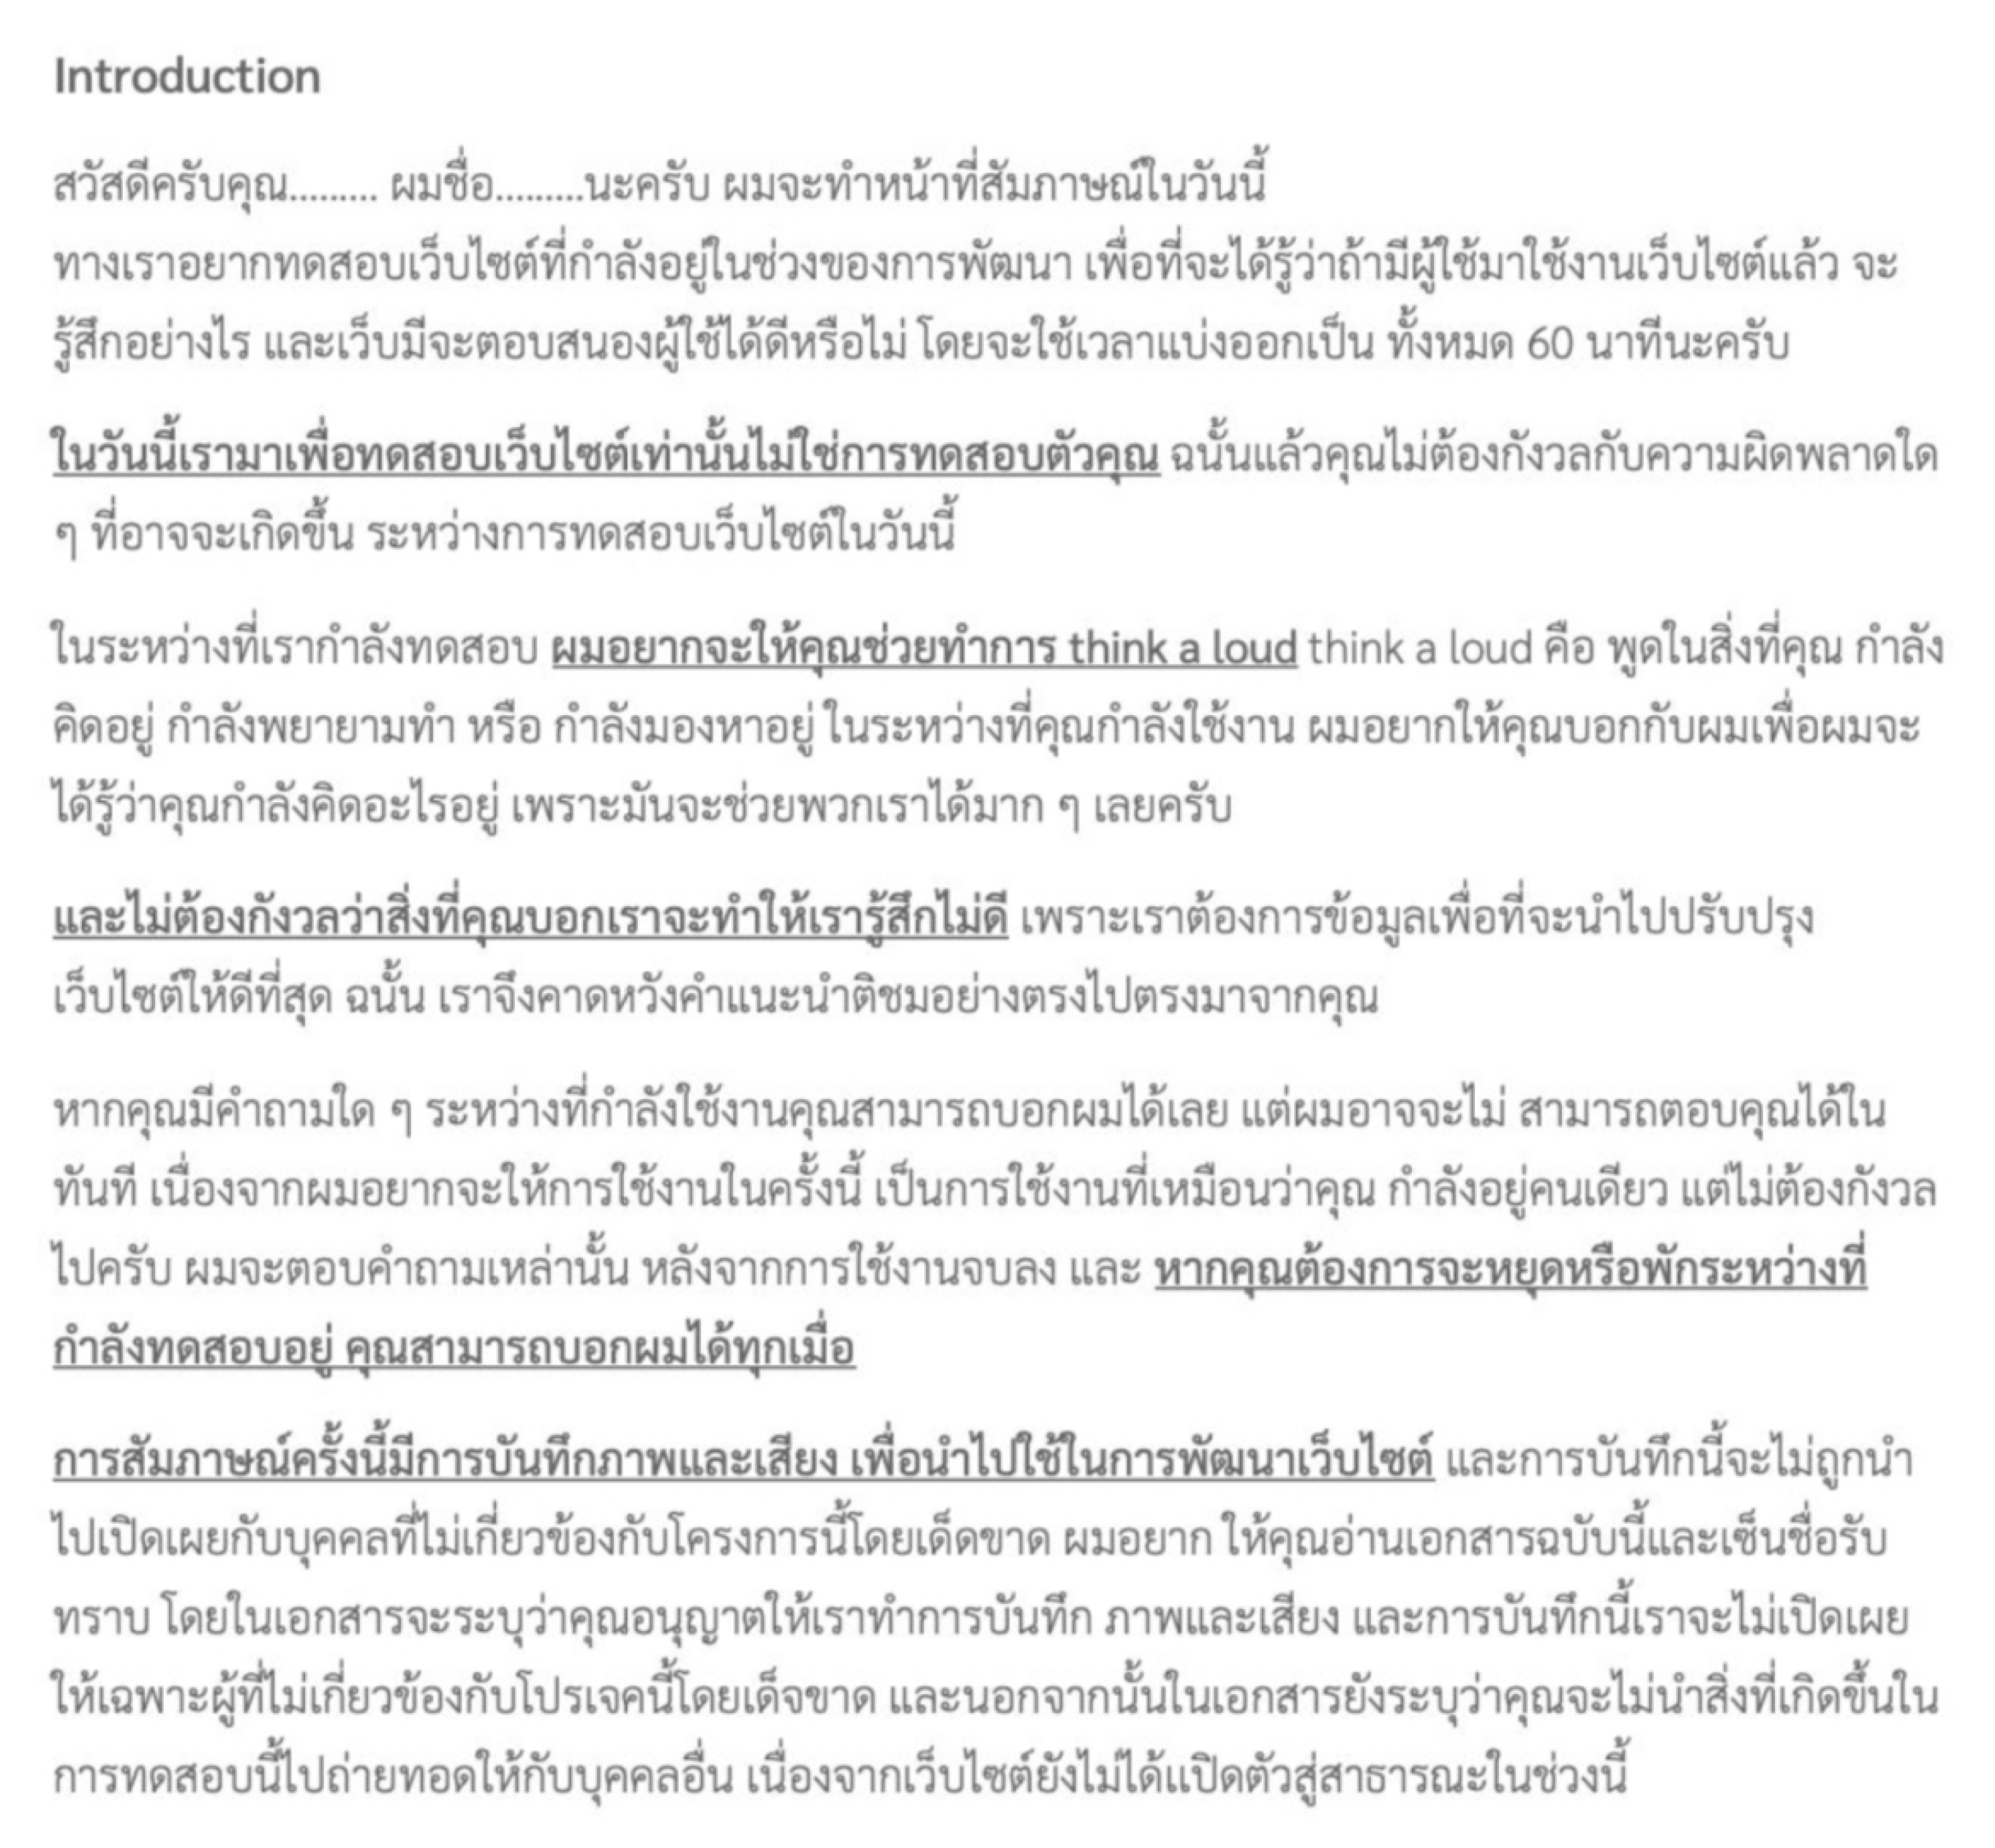
\includegraphics[width=14cm]{./figure/UT/ScriptUT.png}}
        \caption{รูปแสดงบทพูดสำหรับการดำเนินการทดสอบ}\label{fig:ScriptUT}
    \end{figure}
    \item \textbf{การวัดผลเชิงปริมาณ} : \href{https://forms.gle/cRmAQGtgpfCHbK5u8}{แบบสอบถามเพื่อวัดผลเชิงปริมาณ}
\end{enumerate}
\subsection{การดำเนินการทดสอบ}
\begin{enumerate}
    \item \textbf{ข้อกำหนดในการทดสอบ}
    \begin{enumerate}
        \item \textbf{กระตุ้นให้ผู้ร่วมทดสอบพูดในสิ่งที่กำลังคิดอยู่} เพื่อให้สามารถสังเกตความเข้าใจในการใช้งานของผู้เข้าร่วมการทดสอบได้มากขึ้น
        \item \textbf{ไม่ชี้นำระหว่างทำการทดสอบ} เพื่อให้การทดสอบเปรียบเสมือนการใช้งานจริงมากที่สุด
        \item \textbf{ไม่อธิบายการใช้งาน} เพื่อทดสอบการใช้งานของผู้ใช้โดยไม่มีการสอนวิธีการใช้มาก่อน
    \end{enumerate}
    \item \textbf{การจดบันทึกระหว่างการทดสอบ}
    \begin{figure}[H]\centering
        \fbox{\includegraphics[width=14cm]{./figure/UT/NoteTaking.png}}
        \caption{รูปแสดงการจดบันทึกระหว่างการทดสอบ}\label{fig:NoteTaking}
    \end{figure}
\end{enumerate}
\subsection{วิเคราะห์ผลการทดสอบ}
\begin{enumerate}
    \item \textbf{เก็บรวมรวมปัญหาระหว่างการทดสอบ} โดยแบ่งปัญหาออกเป็นของแต่ละฟีเจอร​์ ดังนี้
    \begin{figure}[H]\centering
        \fbox{\includegraphics[width=14cm]{./figure/UT/GateringIssue.png}}
        \caption{รูปแสดงการจดบันทึกปัญหาที่พบ}\label{fig:GateringIssue}
    \end{figure}
    \item \textbf{จัดประเภทของปัญหา}
    \begin{figure}[H]\centering
        \fbox{\includegraphics[width=14cm]{./figure/UT/Groping.png}}
        \caption{รูปแสดงการจัดประเภทของปัญหา}\label{fig:Groping}
    \end{figure}
    \item \textbf{นิยามประเภทของปัญหา}
    \begin{figure}[H]\centering
        \fbox{\includegraphics[width=14cm]{./figure/UT/CreateTheme.png}}
        \caption{รูปแสดงการนิยามประเภทของปัญหา}\label{fig:CreateTheme}
    \end{figure}
    \begin{enumerate}
        \item \textbf{Career Prediction (ทำนายสายอาชีพ)}
              \begin{itemize}
                \item ไม่มั่นใจว่าต้องกรอกข้อมูลเป็นภาษาอะไร
                \item ไม่ได้ใช้เรซูเมในการกรอก
                \item ไม่มั่นใจในการกรอกข้อมูลส่วนต่าง ๆ 
                \item กรอกสิ่งที่คาดไม่ถึง
                \item กดปุ่มระหว่างรอผลทำนาย
                \item สับสนตอนดูผลทำนาย
              \end{itemize}
        \item \textbf{Career Insight (ข้อมูลเชิงลึกของสายอาชีพ)}
              \begin{itemize}
                \item ไม่ทราบว่าสามารถดูประวัติการทำนายอื่น ๆ ได้จากอาชีพนี้
                \item พบปัญหาการใช้ส่วนที่แสดงทักษะ
                \item สับสนการแสดงกราฟและทักษะ
                \item ไม่ได้กดเข้าไปดูสายใยอาชีพต่อ
              \end{itemize}
        \item \textbf{Career Exploration (สายใยอาชีพ)}
              \begin{itemize}
                \item ไม่ทราบว่าสามารถกดเพื่อดูทักษะของอาชีพที่แสดงอยู่ได้
                \item Node ของทักษะทับกัน
              \end{itemize}
    \end{enumerate}
    \item \textbf{ลำดับความสำคัญของปัญหาพี่พบ}
    \begin{figure}[H]\centering
        \fbox{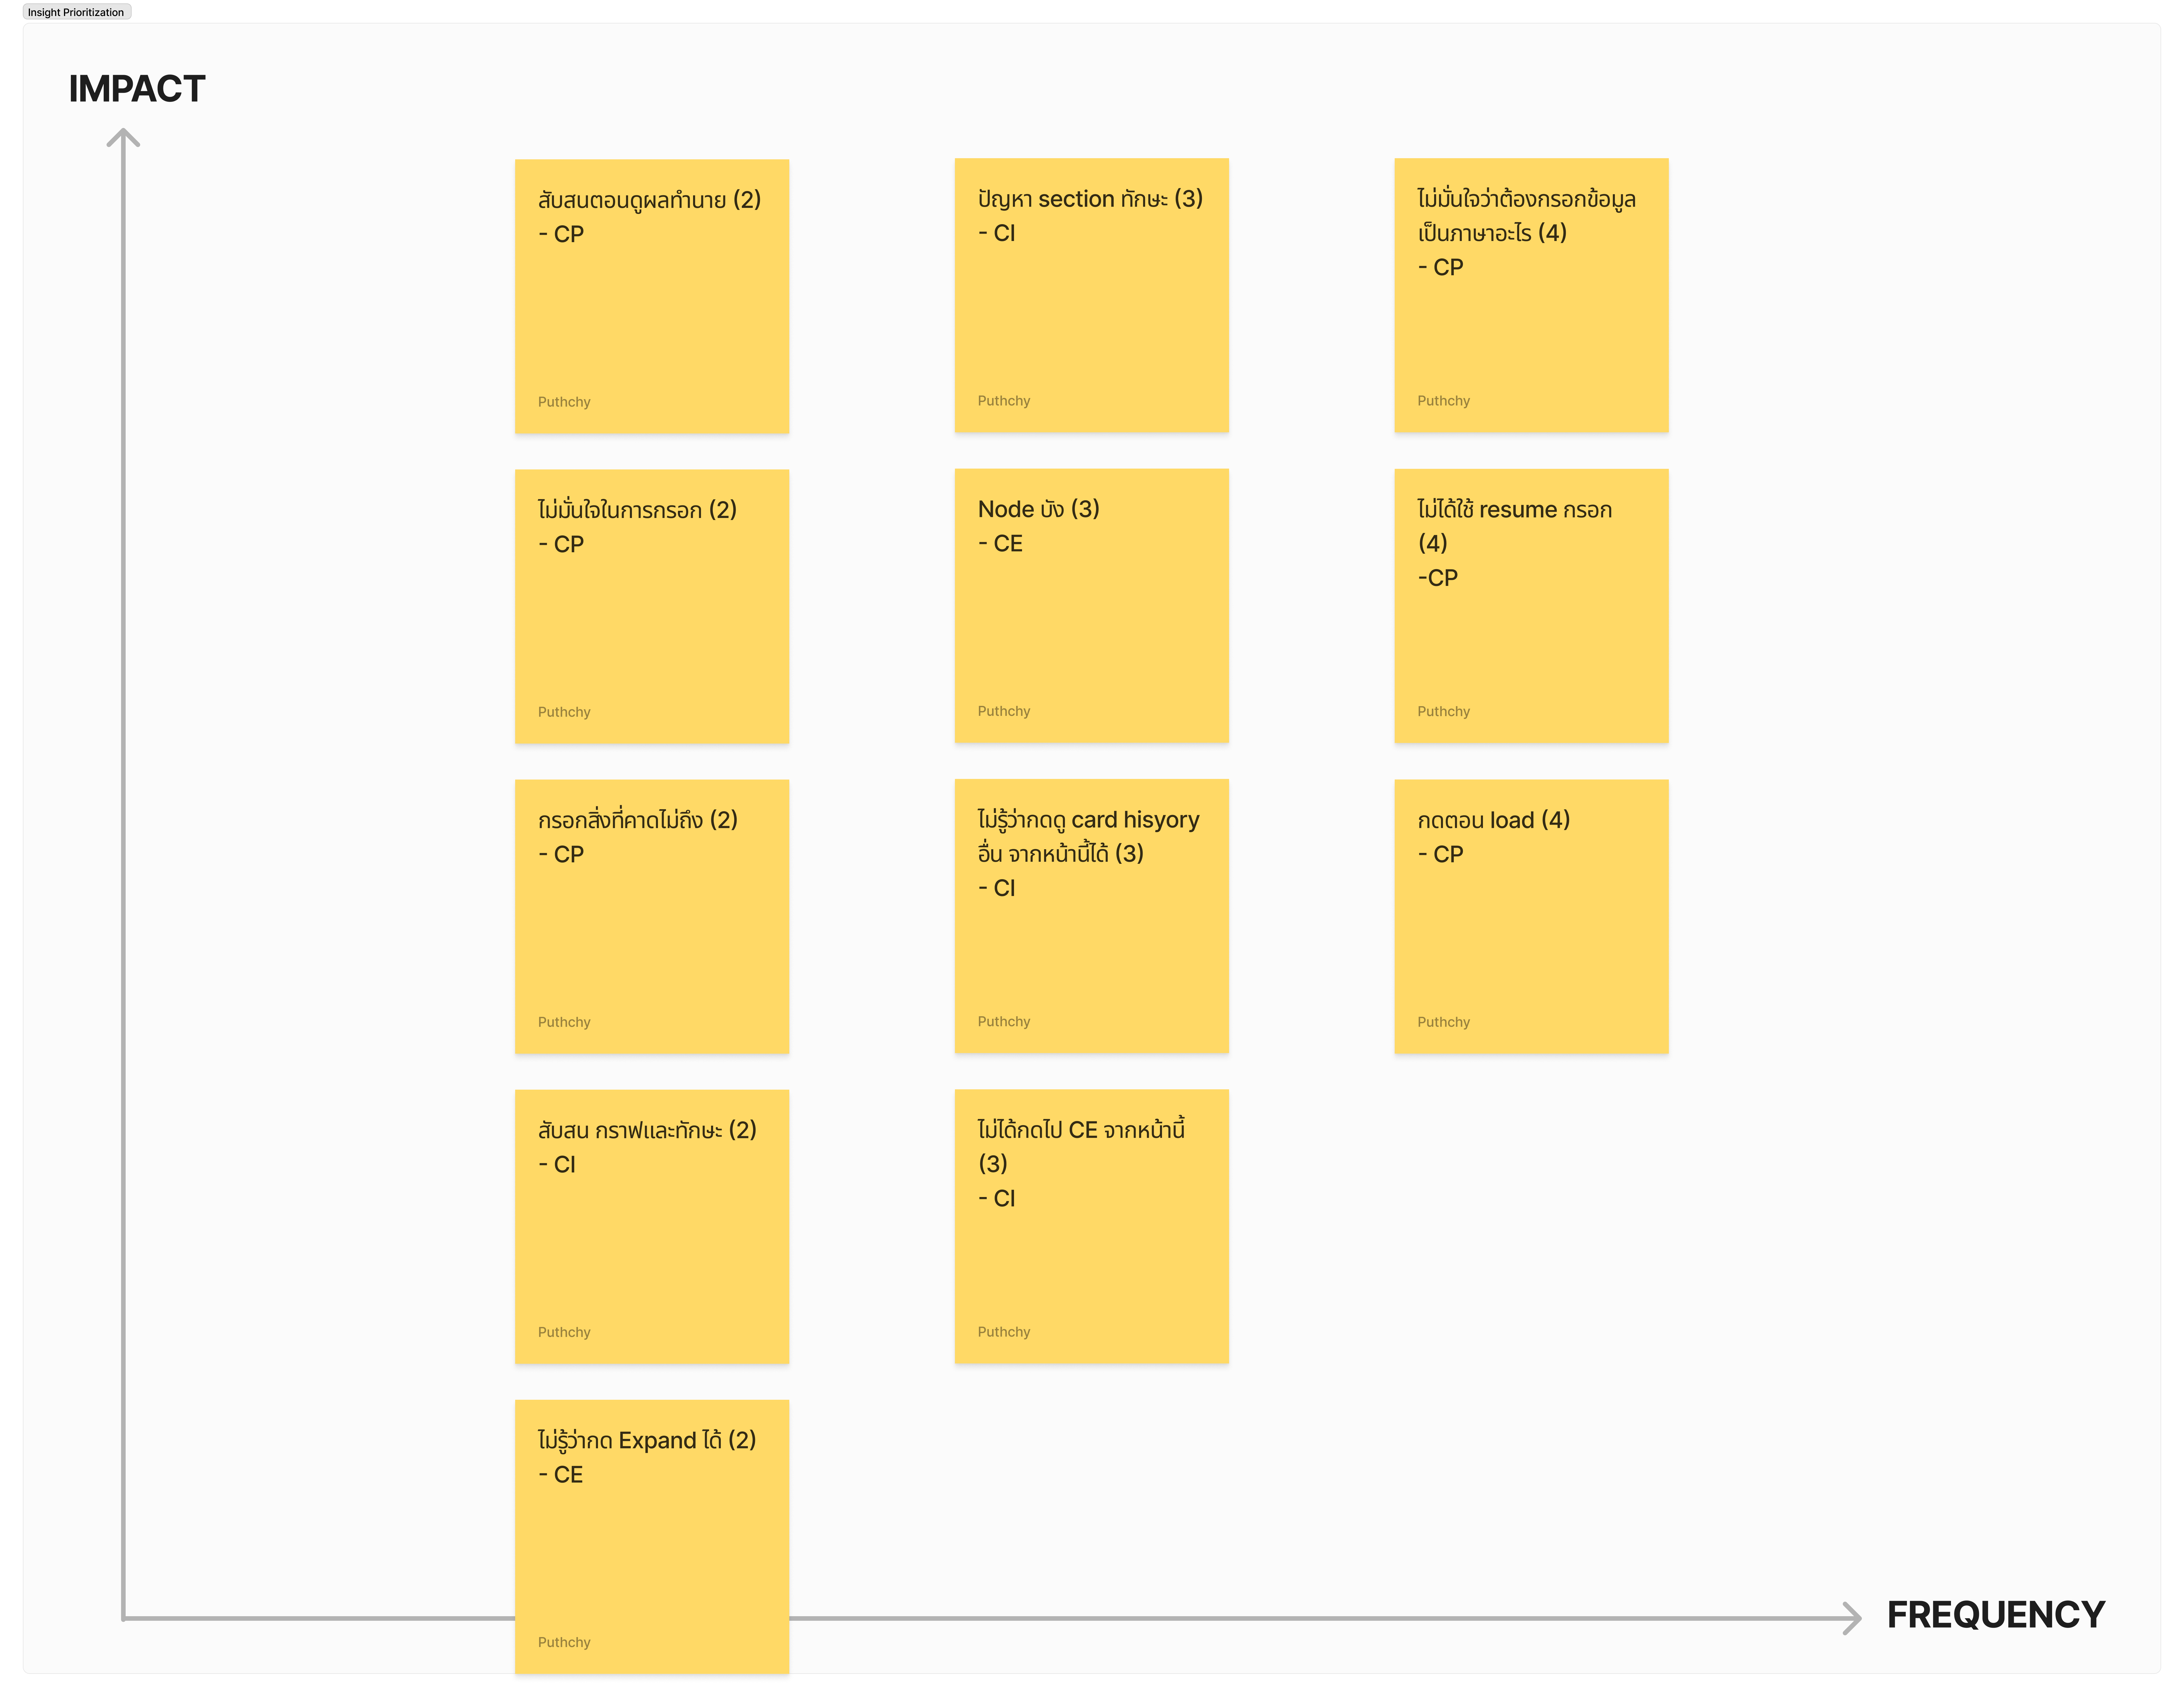
\includegraphics[width=14cm]{./figure/UT/PrioritizeUT.png}}
        \caption{รูปแสดงการเรียงลำดับความสำคัญของปัญหาพี่พบ}\label{fig:PrioritizeUT}
    \end{figure}
    \item \textbf{Create recommendations.}
    \begin{table}[H]
        \caption{แนะนำแนวทางวิธีการแก้ไขปัญหา}
        \label{tab:recommendationsUT}
        \begin{tabularx}{\textwidth}{|l|X|l|X|l|}
        \hline
        \textbf{issue type} & \textbf{issues}                                        & \textbf{page}      & \textbf{recommendations}                                      & \textbf{ease of fixing} \\ \hline
        unclear context     & ไม่มั่นใจว่าต้องกรอกข้อมูลเป็นภาษาอะไร         & Career Prediction  & มีข้อความระบุให้กรอกข้อมูลเป็นภาษาอังกฤษ                      & Medium                  \\ \hline
        unclear context     & ไม่ได้ใช้ resume กรอก                           & Career Prediction  & แบ่ง section การกรอกให้ละเอียดมากขึ้น                         & Difficult               \\ \hline
        not disable button  & กดตอน load                                    & Career Prediction  & ปิดการใช้งานปุ่มระหว่างการรอโหลด                              & Easy                    \\ \hline
        string matching     & ปัญหา section ทักษะ                           & Career Insight     & นำเทคนิคการตรวจจับคำที่ดีขึ้นมาใช้                            & Difficult               \\ \hline
        technical issue     & Node บัง                                       & Career Exploration & ทำ Auto Layout ให้กับ Node                                    & Medium                  \\ \hline
        user interface      & ไม่รู้ว่ากดดู card history อื่น จากหน้านี้ได้  & Career Insight     & ย้าย section ของการเลือกการ์ดมาไว้ในส่วนที่มองเห็นง่ายกว่านี้ & Medium                  \\ \hline
        user interface      & ไม่ได้กดไป CE จากหน้านี้                      & Career Insight     & ทำ section แนะนำให้ไปดูสายใยอาชีพให้ดึงดูมากกว่านี้           & Medium                  \\ \hline
        user interface      & สับสนตอนดูผลทำนาย                              & Career Prediction  & ลดจำนวนปุ่ม, ทำเป็น save อัตโนมัติ                            & Medium                  \\ \hline
        unclear context     & ไม่มั่นใจในการกรอก                           & Career Prediction  & ยกตัวอย่างทักษะให้มากและชัดเจนมากกว่านี้                      & Medium                  \\ \hline
        ML limitation       & กรอกสิ่งที่คาดไม่ถึง                        & Career Prediction  & เทรนข้อมูลเพิ่ม                                               & Difficult               \\ \hline
        user interface      & สับสน กราฟและทักษะ                           & Career Insight     & เขียนอธิบายกราฟว่าเชื่องโยงกับทักษะอย่างไร                    & Medium                  \\ \hline
        user interface      & ไม่รู้ว่ากด Expand ได้                     & Career Exploration & สร้าง tooltips สำหรับการใช้งาน                                & Medium                  \\ \hline
        \end{tabularx}
        \end{table}
\end{enumerate}
